%
% TODO: 
% Abbildungsreferenzen werden nicht gesetzt!!!!
% Anhänge referenzieren
%
\documentclass[11pt]{scrartcl}

% own geometry
%\usepackage[a4paper, left=3cm, right=3cm]{geometry}

\usepackage[ngerman]{babel} 
\usepackage[utf8]{inputenc} 
\usepackage[T1]{fontenc}
\usepackage{graphicx}
\usepackage{color}
\usepackage{xcolor}
\usepackage{hyperref}

% setup of source code listings
\usepackage{listings}
%\usepackage{courier}
\usepackage{caption}
\lstset{
	basicstyle=\footnotesize\ttfamily,	% default font
	numbers=left,						% line numbers placement
	numberstyle=\tiny,					% line numbers style
	%stepnumber=2,						% line number padding
	numbersep=5pt,						% padding between line numbers and code
	tabsize=2,							% 
	extendedchars=true,         
	breaklines=true,						% line breaks 
	keywordstyle=\color{red},
	frame=b,
	stringstyle=\color{white}\ttfamily,	% color of strings in code
	showspaces=false,					% visualize spaces
    showtabs=false,						% visualize tabs
    xleftmargin=17pt,
	framexleftmargin=17pt,
	framexrightmargin=5pt,
	framexbottommargin=4pt,
	showstringspaces=false				% visualize spaces in strings        
 }
 
 \lstloadlanguages{% Check docs for further languages ...
         C,
         C++
 }

\DeclareCaptionFont{white}{\color{white}}
\DeclareCaptionFormat{listing}{\colorbox{gray}{\parbox{\textwidth}{#1#2#3}}}
\captionsetup[lstlisting]{format=listing,labelfont=white,textfont=white}

% layout the box
%\DeclareCaptionFormat{listing}{\colorbox[rgb]{0.43, 0.35, 0.35 {\parbox{\textwidth}{\hspace{15pt}#1#2#3}}}

% layout the caption ontop of code
\captionsetup[lstlisting]{format=listing,labelfont=white,textfont=white, singlelinecheck=false, margin=0pt, font={bf,footnotesize}}

% Document begins now
\begin{document}

\author{%
	Martin Helmich \small(\href{mailto:martin.helmich@hs-osnabrueck.de}{martin.helmich@hs-osnabrueck.de})\\%
	Oliver Erxleben \small(\href{mailto:oliver.erxleben@hs-osnabrueck.de}{oliver.erxleben@hs-osnabrueck.de})\\ \\%
	%
	Hochschule Osnabr"uck \\%
	Ingenieurswissenschaften und Informatik \\%
	Informatik - Mobile und Verteilte Anwendungen }

\title{
\includegraphics[scale=0.75,keepaspectratio]{img/hs_os.png}\linebreak \linebreak
OpenMP [Working DRAFT]}

\maketitle
\thispagestyle{empty}
\tableofcontents

\pagebreak
% set new page style
\pagestyle{plain}
% hoooray page 1! begins 
\setcounter{page}{1} 

\section{OpenMP} Open Multi-Processing (kurz: OpenMP) ist eine Programmierschnittstelle
f"ur die Sprachen C/C++ und Fortran, welche seit 1997 von unterschiedlichen Hardware- und Compilerherstellern entwickelt wird. Ziel von OpenMP, welches mittlerweile den
Versionsstand 3.1 erreicht hat, ist es ein portables und zugleich paralleles
Programmiermodell f"ur Shared-Memory-Architekturen\footnote{Shared-Memory-Architektur: } zur Verf"ugung zu stellen. Es setzt sich aus Compilerdirektiven, Bibliotheksfunktionen und Umgebungsvariablen zusammen. Anders als viele alternative Ansätze zur Parallelisierung von Programmen sind nur wenige Änderungen an sequenziellen Programmen notwendig um parallele Abläufe zu implementieren. Auch die Lesbarkeit des parallelisierten Quelltextes wird im Vergleich zu anderen alternativen Ansätzen stark verbessert. \textit{(Vgl. \cite{omp08} Kapitel 1: Einf"uhrung)}

Ein weiteres Plus f"ur den Einsatz von OpenMP ist die weite Verbreitung von Multi-Core-Rechnern und die Implementierung in vielen verbreiteten Compilern. So ist OpenMP im GCC seit der Version 4.2, im Visual Studio C/C++ Compiler seit der Version 2005 oder im Intel C/C++-Compiler seit Version 8 verf"ugbar. Compiler die keine OpenMP-Unterst"utzung bieten, ignorieren aufgrund der Pragma-Compilerdirektiven die Ausf"uhrung als parallelisierte OpenMP-Implementierung, was zu einer guten Portabilität f"uhrt.

Ursprünglich wurde OpenMP für den Bereich High Performance Computing entwickelt, wo Programmcode meist viele Schleifen enthält. Demnach ist die Parallelisierung von Schleifen die Hauptaufgabe von OpenMP und die meisten Vorteile können an dieser Stelle von OpenMP aufgezeigt werden. 
% TODO: Beispiel einfügen??

\subsection{Merkmale von OpenMP}

Mit OpenMP wird ein hoher \textbf{Abstraktionsgrad} erreicht, da Threads nicht durch einen Programmierer initialisiert, gestartet oder beenden werden m"ussen. Wie bereits in der Einf"uhrung erwähnt, beitet OpenMP eine gute \textbf{Portabilität} des Programms an, zum einen ist OpenMP in vielen Mainstream-Compilern implementiert, zum anderen können Compiler ohne OpenMP-Unterst"utzung das Programm ohne Veränderung kompilieren, da die Compilerdirektiven durch Pragmas eingesetzt und ignoriert werden können. Auch bleibt der sequenzielle Programmcode vollständig erhalten, wenn nicht mittels OpenMP kompiliert wird. Der Quelltext kann somit \textbf{Schrittweise parallelisiert} werden. 

\subsection{Ausführungsmodell}

Die parallele Ausf"uhrung erfolgt durch Threads auf dem
Fork-/Join\footnote{Fork/Join:}-Ausf"uhrungsmodell. Zu Beginn eines Programms ist nur ein Thread aktiv, der sog. \textit{Master Thread}. Sobald bei der Programmausf"uhrung die Direktive \textit{\#pragma omp parallel \{ ... \} } erreicht wird, gabelt sich die
Ausf"uhrung in Threads auf. Die erstellten Threads werden als \textit{team of threads}
bezeichnet\footnote{Die Implementierung von OpenMP entscheidet "uber die Art der Threads die erstellt werden. Es könnten Threds auf Basis der PThreads-Bibliothek oder aber auch als vollwertige Shared-Memory-Prozesse umgesetzt sein.}. F"ur OpenMP, bzw. der Entwicklung mit OpenMP stellen Threads einen Kontrollfluss mit gemeinsamen Adressraum dar.

Die schließende geschweifte Klammer ist zudem ein Synchronisationspunkt, andem das team of threads auf alle Teammitglieder wartet. Die Abbildung \ref{join_fork_model} stellt einen möglichen Ablauf mit OpenMP dar.

Sofern nicht anders angegeben verwenden alle Threads eines Thread-Teams einen gemeinsam genutzten Adressraum und können somit auf alle Variablen eines parallen Codeabschnitts zugreifen, über die auch die Kommunikation zwischen den Threads ermöglicht wird. Folgende Klauseln für Variablen können eingesetzt werden:

\begin{itemize}
\item \textit{shared}/\textit{private}: Threads können explizit als gemeinsame Variable oder für jeden Thread private Variable deklariert werden.
\item \textit{firstprivate}/\textit{lastprivate}: Diese Klauseln erlauben die Initialisierung, bzw. Finalisierung der Variable beim Ein- und Austritt in oder aus einem parallen Bereich.
\item \textit{default}: Das Standardverhalten kann verändert werden. % TODO nochmal prüfen
\item \textit{reduction}: Eine spezielle gemeinsam genutzte Variable über die mehrere Threads Wrte zusammentragen können.
\end{itemize}


\begin{figure}[h!]
\centering
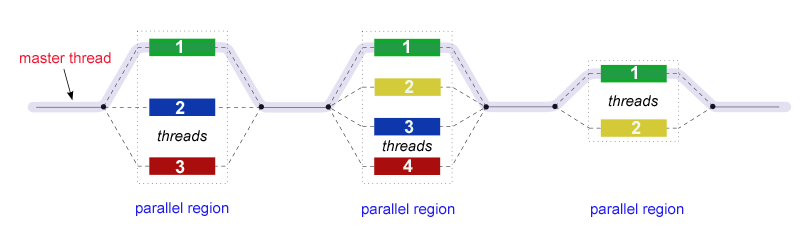
\includegraphics[width=1.0\textwidth]{img/fork_join.png}
\label{join_fork_model}
\caption{Fork-Join-Prinzip}
\protect{\textit{Entnommen aus OpenMP Tutorial} (siehe \cite{openmptut})}
\end{figure} 

\subsection{Parallelisierung von Schleifen} 
Nach der Klassifikation von Flynn kann OpenMP als Single Programm Multiple Data (SPMD) beschrieben werden. Demnach führt jeder Thread der gestartet wurde den Schleifenblock aus. Dabei hat jeder Thread seine eigene Iteration und Teilmenge von Daten.\textit{(Vgl. siehe \cite{omp08}, Kapitel 3.1: Parallelität auf Schleifenebene)}

Ein team of threads wird mittels \textit{\#pragma omp parallel} gestartet. Zur Veranschaulichung sei das Listing \ref{parallelExample} gegeben. 

\lstinputlisting[caption= pragma omp parallel - Beispiel, label=parallelExample]{../src/1_3_example/parallel.c}
Die For-Schleife in Zeile 8 wird von allen vom System zur Verfügung stehenden Threads ausgeführt. Allerdings teilen sich die Threads nicht die Arbeit, sondern jeder Thread führt die Schleife komplett für sich aus. Um eine Schleife parallel auszuführen, muss über eine weitere Direktive, wie in Listing \ref{parallelForExample} zu sehen, eingefügt werden. 

\lstinputlisting[caption= pragma omp parallel for - Beispiel, label=parallelForExample]{../src/1_3_example/parallelfor.c}
In diesem Beispiel wird der zu parallelisierende Bereich eine Variable \textit{tid}, die threadId, übergeben. Jeder Thread erhält diese Variable, die nicht gemeinsam genutzt werden kann (private). Mittels \textit{\#pragma omp for} wird dem Compiler mitgeteilt das die darauffolgende Schleife parallel durch das team of threads  im parallelen Bereich ausgeführt werden soll.

Als Vorraussetzung für parallelisierbare Schleifen fordert OpenMP, dass Schleifen in kanonischer Form geschrieben sein müssen. Die kanonische Form liegt wenn folgende Bedingungen erfüllt sind: 
\begin{itemize}
\item Anzahl der Schleifendurchläufe muss berechnbar sein und darf sich innerhalb des Schleifenblocks nicht ändern. Ebenso dürfen sich Start und Endwert während des Schleifendurchlaufs nicht ändern.
\item Es sind nur boolsche Vergleichoperator im Schleifenkopf erlaubt.
\item Das Inkrement im Schleifenkopf darf nur aus Addition oder Subtraktion inkrementiert oder dekrementiert werden. 
\item \textbf{break}-Anweisungen dürfen nicht im Schleifenrumpf verwendet werden. Allerdings kann eine Iteration durch eine \textbf{continue}-Anweisung übergangen werden oder das gesamte Programm mittel \textbf{exit} verlassen werden.
\end{itemize}

\subsection{Synchronisation} 

Wie im Kapitel 1.2 bereits erläutert wird ein team of threads durch ihren gemeinsamen Adressraum synchronisiert. Dabei ist die Reihenfolge der Bearbeitung der Arbeit nicht "vorhersehbar". Um einen kritischen Adressraum innerhalb eines parallelen Abschnitts zu kennzeichnen, bietet OpenMP ein weitere Direktive an: \textit{\#pragma omp critical \{ ... \}}. Der von der Klammer umschlossene Code wird demnach von nur einem Thread ausgeführt. 

%\subsection{Abschnitte und Aufgaben}

\pagebreak % first part ends

%\section{Vergleich mit TBB und anderen?!}

%\pagebreak % second part ends

\section{Vergleich eines parallelen OpenMP-Programms mit einem vergleichbaren auf Grundlage der Intel TBB}

\subsection{Vorgehen}

Die Implementierung und Parallelisierung mittels OpenMP wird beispielhaft in diesem Dokument aufgezeigt. Als Grundlage für die Implementierung wird eine optimierte Version des Quelltexts der Parallelisierungsaufgabe (siehe Anlage !?!?!?!) aus dem Intel Programmierwettbewerb von November 2012 verwendet. Die Aufgabenstellung der Programmieraufgabe ist als Anhang !?!?! beigefügt. 

\subsection{Auftretende Probleme}

  * Keine Entsprechung für parallel\_do in OpenMP. Vorgehen? (Umformung in rekursive Variante, zu Benchmark-Zwecken sequentiell arbeiten lassen?)
  * Tasks nicht in allen Compiler-Versionen unterstützt

\subsection{Ergebnisse}

Noch zu bestimmen.

\section{Fazit}

Einfach anwendbar, speziell auf bereits existierenden sequentiellen Code

Funktionale Vor- und Nachteile im Vergleich zur TBB:

  * (-) Parallele While-Schleifen fehlen.
  * (-) Task-Parallelität wurde erst spät in den Standard aufgenommen und steht noch nicht in allen Compiler-Versionen zur Verfügung (verflucht mögt ihr sein, Apple!)
  * (+) Mehr Möglichkeiten zur Synchronisation (z.B. durch Barriers)
  * (-) Keine Threadsicheren Datenstrukturen wie in der TBB (die entsprechenden ADT der TBB können jedoch auch unter OpenMP verwendet werden)
  * (-) TBB hat verschiedene Datentypen zur Synchronisierung (Normale Mutexe, Spin-Mutexe, Queue-Mutexe, und alles nochmal als RW-Variante), OpenMP kennt nur einfache Locks.

\pagebreak % third part ends

\thispagestyle{empty}
\listoffigures

\listoftables

\lstlistoflistings

\begin{thebibliography}{3}
	\bibitem{omp08} S. Hoffmann, R. Lienhart: OpenMP - Eine Einf{\"u}hrung in die parallele Programmierung in C/C++
	
	\bibitem{openmptut} Blaise Barney, Lawrence Livermore National Laboratory: OpenMP Tutorial \\ https://computing.llnl.gov/tutorials/openMP/ \\ \textit{abgerufen am 24.11.2012}
\end{thebibliography}

\end{document}
